\documentclass{sig-alternate}
\usepackage{amsmath}
\usepackage{hhline}
%\documentclass{ueacmpstyle}


\begin{document}
\title{Experimental Project: search experiments}
\author{
100036248 or C.A.Irvine
}
\maketitle
	\section{Introduction} \label{sec:intro}
	Modern Information Retrieval (IR) systems, by definition, are expected to return documents that are relevant to the supplied Search Query. What are the necessary steps to achieving this goal? What tools will be employed? How do we test and improve an IR system?
	
	This paper aims to answer these questions, providing the steps needed to build an accurate IR system. By the end, we will have the knowledge needed to build and continuously improve a retrieval system that can be applied to domains of any size. For the purposes of this paper, we will be building the system using the portal.uea.ac.uk domain.
	
	\section{Initial System} \label{sec:base}
	The base IR system can be divided into two sub-systems: indexing and retrieval.
	
	The base retrieval system is not accurate, when a relevant document is mentioned, it means the system believes it to be relevant. In reality, the returned documents are rarely relevant for this base system.
	
	For ease, this system and subsequent systems will print to the command line, allowing the focus of this experiment to remain solely on returning relevant documents, see Figure \ref{fig:retriever-output}.
	
		\subsection{Indexing} \label{sec:base-index}
		The indexing subsystem takes a web domain and uses a \textbf{NIST PCcrawler web spider program} (\cite{NIST}). Each document is cleaned of all HTML, numbers, special characters and contractions. The `clean' document text is separated into tokens and from there a vocabulary of unique terms is generated. For every term in the vocabulary; the occurrence of that term is counted for each document, this creates the postings table.
		
		\subsection{Retrieval} \label{sec:base-retrieval}
		The retrieval subsystem reads the Search Query supplied by the user, `cleans' it using the same method as indexing (Section \ref{sec:base-index}), and then uses the postings table to generate the \textbf{Term Frequency * Inverted Document Frequency (TF*IDF)} score for each word in the query and each document relevant to that word. The scores are combined and all relevant documents are ordered. The top 10 documents are displayed to the user. 
		
	\begin{figure}
		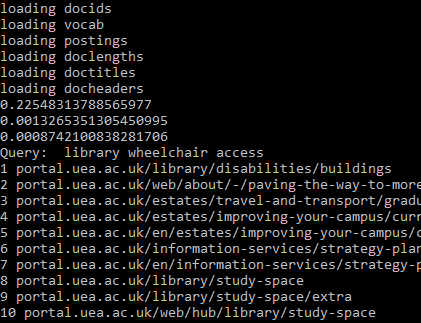
\includegraphics[width=1\linewidth, height=4cm,]{retrieverOuput.PNG}
		\caption{Output produced from the retrieval subsystem, stemming (see Section \ref{sec:enh-stemming)} and weighting (see Section \ref{sec:enh-weighting})is present in this system}
		\label{fig:retriever-output}
	\end{figure}
		
	\section{TF*IDF} \label{sec:TFIDF}
	As discussed in Section \ref{sec:base-retrieval}, the retrieval system uses TF*IDF to rank the relevance of each document. TF*IDF returns a score between 0 and 1, 1 being entirely relevant. The formula for TF*IDF is below ((\cite{modernIR}), (\cite{IntroIR}):
	\begin{gather*}
		TF*IDF \ = \ (log\textsubscript{10}\frac{N}{n\textsubscript{i}}) \times (\frac{freq\textsubscript{i,j}}{P\textsubscript{j}}) \\
		freq\textsubscript{i,j} = Frequency \ of \ term \ i \ in \ document \ j \\
		P\textsubscript{j} = Number \ of \ terms \ in \ document \ j \\
		N = Number \ of \ documents \ in \ collection \\
		n\textsubscript{i} = Number \ of \ documents \ containing \ term \ i
	\end{gather*}
	
	\section{Enhanced System} \label{sec:enh}
	Taking the system discussed previously (see Section \ref{sec:base}) as a base, we can drastically enhance the quality of the retrieved documents with a few simple additions; namely stemming and weighting. 
	
		\subsection{Stemming} \label{sec:enh-stemming}
		Stemming is the process of removing prefixes and suffixes from words to leave the roots. This allows words to be generalised and prevents natural speech patterns interfering with both the indexing and retrieval subsystems (as the search queries are `cleaned' in the same manner as the indexing).
		
		The \textbf{Natural Language ToolKit (NLTK)} (\cite{NLTK}) provides several stemming modules. Each module stem words to different levels. Stemming carries a risk that the word is stemmed incorrectly and will become irrelevant to all searches (\cite{stemming}). Three modules were tested; Snowball, PorterStemmer and WordNet (listed in order to strength). 
		
		Three vocabularies were generated, one for each module, for the same 30 documents. Each word that was not a recognisable English word was counted for each module. The lightweight, WordNet Lemmatizer stemmer was chosen, as it had the least amount of incorrect words.
		
		\subsection{Weighting} \label{sec:enh-weighting}
		Weighting prioritises documents that mention search terms in Titles, Headers and in the opening paragraph of the document. Further alteration to the indexing subsystem is needed, but also requires the retrieval subsystem is adapted, to implement Weighting.
		
		The indexing subsystem must copy the tokens that are in the \textbf{<title>}, \textbf{<h>} and \textbf{<meta content=``''>} tags are stored in their own files. In addition to this, the \textbf{first thirty tokens} for each document is stored separately as well. 
		
		In the retrieval subsystem, these separated files are read in and searched for the Search Query Terms. If they are found in the files an additional multiplier is applied to that term's IDF value (see Section \ref{sec:TFIDF}).
	
	\section{Evaluation} \label{sec:eval}
	At each stage of the system's development, the precision was tested by running the same query - ``multifaith centre opening times'' - and comparing the precision to the base. We can see from Figure \ref{fig:comparison-line} that the Final System (which incorporates both Weighting and Stemming) is significantly superior to the base system, however precision does drop and plateau at the Weighted System level.
	
	\begin{figure}
		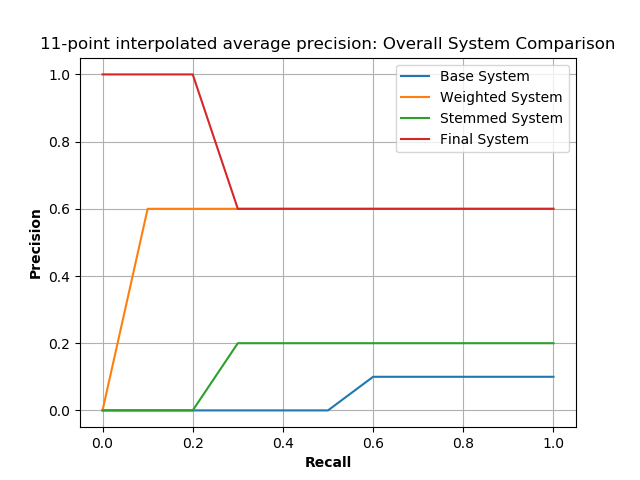
\includegraphics[width=1\linewidth, height=5cm,]{p11-overall.PNG}
		\caption{Line graph showing the 11-point interpolated average precision for each stage of the system.}
		\label{fig:comparison-line}
	\end{figure}

		\subsection{Set Query Evaluation} \label{sec:eval-setQeval}
		The supervisor of this project supplied a list of 10 queries for the system to be evaluated with. The top 100 returned documents were analysed by a python script was written to generate statistical and graphical analysis on these queries. One of the critical statistics returned by the script was the \textbf{Average Precision Value (APV)}. Queries 1, 5, 8 and 10 are presented in Table \ref{tab:apv} because collectively they are the best, worst and most inaccurate results produced by the final system. They average is also presented for comparison.
		
		\begin{table}
			\centering
			\caption{Table showing select Average Precision Values (to 3 sf) from a set of 10 Queries, in addition to the Average of the 10 Queries}
			\label{tab:apv}
			\begin{tabular}{|l|c|c|c|c|c|}
				\hline
				\textbf{}                                                                           & \textbf{Q1} & \textbf{Q5} & \textbf{Q8} & \textbf{Q10} & \textbf{Average} \\ \hhline{|=|=|=|=|=|=|}
				\textit{\begin{tabular}[c]{@{}l@{}}Average\\ Precision\\ Value (3 sf)\end{tabular}} & 0.321       & 0.691       & 0.929       & 0.148        & 0.638  \\ \hline         
			\end{tabular}
		\end{table}
	
		\subsection{Q5 Investigation} \label{sec:eval-Q5}
		As we take a closer look into the 68 documents returned by Query 5: \textbf{Neil Ward} we start to understand why Q5 had an above average APV. 52 of the 68 documents mention a different Neil within the portal.uea.ac.uk domain, meaning that the majority of returned documents are irrelevant to the User. The first 6 results returned directly concern \textbf{Neil Ward}, so the User would likely be satisfied by the returned documents.
		
		To improve on this inaccurate result, \textbf{Named Entity Recognition (NER)} tools supplied by NLTK (see Section \ref{sec:enh-stemming}, \cite{NLTK}) can be integrated to the system. This will likely improve other query results.
		
		\subsection{Future Improvements} \label{sec:eval-future}
		In addition to the NER improvement suggested in Section \ref{sec:eval-Q5}, a Graphical User Interface (GUI) could be developed so that the Snippets (mentioned in Section \ref{sec:enh-weighting}) can be displayed. The GUI can also provide a platform for User Feedback so that Relevance Feedback can continuously improve the IR System.
	
	\section{Conclusion}
	In this paper we have learned how to build an Information Retrieval System (see Sections \ref{sec:base}, \ref{sec:TFIDF} and \ref{sec:enh}), using industry standard tools (see Section \ref{sec:enh-stemming}). Then we learned how to evaluate the Information Retrieval System (see Section \ref{sec:eval}), with the aid of a Python Script, looking at Graphs and Statistics to identify areas for improvement within the Information Retrieval System (see Section \ref{sec:eval-Q5}). Finally, additional future improvements for the IR System were suggested with the aim of improving both Accuracy and Usability.

\bibliographystyle{apalike}
\bibliography{IR_CWK_Flyer.bib}  

\end{document}
